\documentclass{beamer}
\usepackage{lsfolien}
\usepackage[english]{babel}

\myfootline{Sustainability, Environment, Management -- Summer Term
  2022}{Hans-Gert Gr\"abe}

\title{On the Notion of a Resource\vskip1em}

\subtitle{Research Seminar in the Module 10-202-2312\\ for Master Computer
  Science}

\author{Prof. Dr. Hans-Gert Gräbe\\
\url{http://www.informatik.uni-leipzig.de/~graebe}}

\date{April 2022}
\begin{document}

{\setbeamertemplate{footline}{}
\begin{frame}
  \titlepage
\end{frame}}

\begin{frame}{Systems and Problem Solving}

The concept of system is a basic mental tool for delimiting and reducing
problems to their essentials.

Such focussing and contextualisation is the prerequisite for further planful
proceeding according to Darrell Mann: 
\begin{itemize}
\item for modelling the problematic situation ("Define"), 
\item for selection of suitable solution tools ("Select"), 
\item for generation of solution proposals ("Generate") and 
\item the assessment and selection of suitable solutions ("Evaluate").
\end{itemize}

D. Mann stops at this mental stage in his book, which of course must still be
followed by the implementation of the solution -- "it is not only about
interpreting the world differently, it is a matter of changing it" (Marx).
\end{frame}

\begin{frame}{The TRIZ Way of Thinking}
\small
  \begin{center}
  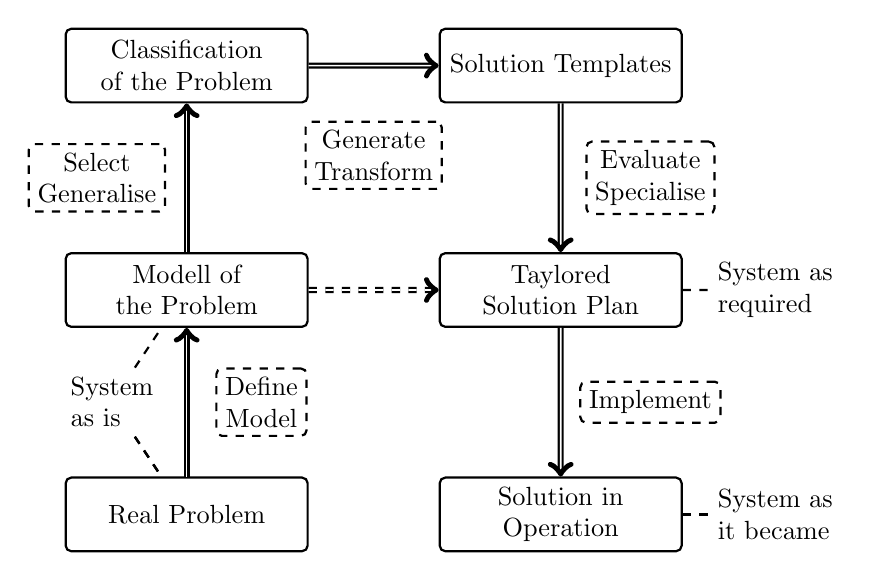
\begin{tikzpicture}[scale=.95,transform shape,
      textbox/.style={draw, text width=3cm, minimum height=2.8em,
        align=center},
      ovalbox/.style={draw, dashed, align=center},
      %>={Triangle[length=0pt 6,width=0pt 5]},
      rounded corners=2pt,line width=.8pt]

    \node[text width=1.1cm] at (-1,1.5) (A0) {System\\ as is};
    \node[textbox] at (0,0) (A1) {Real Problem};
    \node[ovalbox] at (1,1.5) {Define\\ Model}; 
    \node[textbox] at (0,3) (A2) {Modell of the Problem};
    \node[ovalbox] at (-1.2,4.5) {Select\\ Generalise}; 
    \node[textbox] at (0,6) (A3) {Classification of the Problem};
    \node[ovalbox] at (2.5,4.8) {Generate\\ Transform}; 
    \node[textbox] at (5,6) (B3) {Solution Templates};
    \node[ovalbox] at (6.2,4.5) {Evaluate\\ Specialise}; 
    \node[textbox] at (5,3) (B2) {Taylored\\ Solution Plan};
    \node[ovalbox] at (6.2,1.5) {Implement}; 
    \node[textbox] at (5,0) (B1) {Solution in Operation};
    \node[text width=1.8cm] at (8,3) (C2) {System as\\ required};
    \node[text width=1.8cm] at (8,0) (C1) {System as\\ it became};

    \draw[-,dashed] (A0) -- (A1);
    \draw[-,dashed] (A0) -- (A2);
    \draw[-,dashed] (B1) -- (C1);
    \draw[-,dashed] (B2) -- (C2);
    \draw[-,dashed] (A0) -- (A1);
    \draw[-,dashed] (A0) -- (A1);
    
    \draw[double,->] (A1) -- (A2) ;
    \draw[double,->] (A2) -- (A3) ;
    \draw[double,->] (A3) -- (B3) ;
    \draw[double,->,dashed] (A2) -- (B2) ;
    \draw[double,->] (B3) -- (B2) ;
    \draw[double,->] (B2) -- (B1) ;
\end{tikzpicture}
\end{center}
\end{frame}

\begin{frame}{Define}

This first step in Darrell Mann's approach starts with the delineation of an
appropriate systemic context for the study of the problem.
  \begin{itemize}
  \item Delimitation of the system externally against a "living" context as
    \emph{environment}. 
  \item Delineate the system internally -- delineate \emph{components} that
    either already exist (as \emph{artefacts} or as \emph{services}, i.e. also
    "belong to the environment") or are available at the time of assembling
    and operating the system.
  \end{itemize}

This allows concentration on the \emph{internal view} and planning of a
\emph{functional solution} to the problem.
\end{frame}

\begin{frame}{TRIZ Concept of the Ideal Machine}

In the TRIZ methodology \emph{functional} properties as "usefulness for
others" are in the foreground.

The terms \emph{usefulness} and \emph{harmfulness} play an important role in
TRIZ alongside the objectives of profitability and efficiency as
socio-cultural guiding principles.

With the concepts of \emph{Ideality} and \emph{Ideal Final Result} a mental
construct of anticipation of the functional properties of a system stands at
the beginning of its genesis.
\begin{block}{Koltze/Souchkov, p. 40}
  The ideal machine is a solution in which the maximum utility is achieved but
  the machine itself does not exist. 
\end{block}
\end{frame}

\begin{frame}{TRIZ Concept of the Ideal Machine}

The ideal machine is therefore \emph{pure functionality} without any
resource-related underpinning.

Nonetheless, that fictitious idea is central to TRIZ, for it develops a strong
orientation towards the intended usefulness and thus has a socio-cultural
guiding effect.

\emph{Machine} here stands very generally for "potentially working solution"
and hence applies also to problem solving in socio-technical systems as
organisations.
\end{frame}

\begin{frame}{Select, Generate, Evaluate}\small

Here Darrell Mann deviates somewhat from my scheme.

My „Generalise“ is rather part of „Define“ but not directed towards modelling
of the given problem, but at finding a \emph{working conceptual
  generalisation}.

„Select“ appropriate tools requires or is interwoven with finding this working
conceptual generalisation.

„Generate“ much depends on a good choice of tools and thus of a working
conceptual generalisation.  Hence the demarcation of the transformation on the
higher level of abstraction is slightly different.  

This also applies to „Specialise“. It is more than mere „Evaluation“ since it
comprises to taylor a general solution template to the given situation.

In both versions the process ends with a \emph{plan} for the implementation of
the solution.

\end{frame}

\begin{frame}{Implement}

This phase does not occur in Darrell Mann's work (and in TRIZ in general) in
such a clear way as it does, for example, in Design Thinking.

But the DT methodological approach is different: the methodological focus is
rather on the multiple rapid (agile) passing through the feedback cycle
between real problem and possible solutions instead of precise planning.

\end{frame}

\begin{frame}{Implement}

Implement in (or after) TRIZ means: 
\begin{itemize}
\item Machine must be "built".
\item Machine must be "deployed" at the given location and "come to life".
\item To do this, the \emph{operating conditions} (import and export) must be
  provided.
\item Which resources are needed (input) and which are made available (output). 
\end{itemize}
\vfill

What are resources in TRIZ? 
\vfill
\end{frame}

\begin{frame}{On the Notion of Resources in TRIZ}

\begin{block}{ARIZ-85C:}
  „Substance Field Resources are substances and fields that are already
  available or are (easily) obtainable according to the conditions of the
  task“.
\end{block}
  
Wessner lists a whole variety of concepts of resources proposed by different
TRIZ schools.  The spectrum ranges from 
\begin{itemize}
\item "a means that can be used to solve a problem" (Souchkov) 
\item to "anything in or around the system that is not being used to its
  maximum potential" (Mann, Salamatov)
\item to the notion of resource as source of a problem itself: "a problem
  always arises, if a needed resource is not present" (Orlov).
\end{itemize}

\end{frame}

\begin{frame}{On the Notion of Resources in TRIZ}\small

In (Koltze/Souchkov, p. 51) a resource is understood as "a means, a tool to
carry out an action or to make a process take place" and equipment, money
funds, raw material, energy or even people (human resources) are mentioned as
examples of resources.\vspace*{-.5em}

Furthermore ressources there are classified according to\vspace*{-1em}
\begin{itemize}
\item \emph{value} (free, not expensive, expensive),
\item \emph{quality} (harmful, neutral, useful),
\item \emph{quantity} (unrestricted, sufficient, insufficient) and
\item \emph{readiness for use} (ready, to be modified, to be developed).
\end{itemize}\vspace*{-1em}

Specific \emph{qualitative} determinations of such "substances and fields" as
resources play almost no role.\vspace*{-.5em}

Qualitative determinations in the sense of the fulfilment of a
\emph{specification} are, however, essential in more complex technical
contexts in order to ensure the \emph{operation} of a specific functional
property, which is to be provided by a systemic context.

\end{frame}

\begin{frame}{What is the Problem?} 

The constructed thing (partial system) that has been taken out must be
(re)placed in the overall context.  But this context can be operated only as a
\emph{unified whole} that cannot be disassembled from an operational point of
view. The whole can only be operated in an assembled state, and this
requirement to be "assembled" does not end at any system boundary either.

It means putting the "dead" partial system (after appropriate preparation)
into a "living" (itself being systemically structured) environment and
"starting it to operate".

\emph{Preparation:} In component software, a distinction is made between
deploy, install and configure as well as an explicit signal to switch from
preparation to operating mode.

\end{frame}

\begin{frame}{What is the Problem?} 

This induces a \emph{further systemic development} of the "living" environment
as a systemic complex, i.e. \emph{the whole changes}.

This requirement later to operate the system must already be present in the
entire (mental) development process.

How does this throughput of substance, energy and information appear in the
TRIZ modelling process?

\end{frame}

\begin{frame}{Operating a Minimal Technical System} 

In the TRIZ notion of a \emph{minimal technical system}, a \emph{tool} acts on
an \emph{object} (workpiece) to be processed in order to transform it into a
\emph{useful product}.

\begin{center}
  \begin{tikzpicture}[scale=.7,transform shape,
      textbox/.style={draw, text width=3cm, minimum height=2.8em,
        align=center},
      >={Triangle[length=0pt 6,width=0pt 5]},
      rounded corners=2pt,line width=.8pt]

    \node[textbox,text width=2cm] at (0,0) (A1) {Tool};
    \node[textbox] at (5,0) (A2) {Processed Object\\ Workpiece};
    \node[textbox,fill=lightgray] at (5,2) (A3) {Useful\\ Product};
    
    \draw[->,line width=2pt,gray] (A1) -- (A2);
    \draw[->,line width=2pt,gray] (A2) -- (A3);
\end{tikzpicture}
\end{center}

The concept of the \emph{ideal system} considers the tool as a purely
functional property, the effect of which to intentionally change the state of
the workpiece to a useful product is achieved without any additional efforts
and any wear of the tool.

In other words, it is not the tool but the \emph{imaginaton of the tool} that
creates the required action in such an \emph{ideal machine}.
\vskip1em
\end{frame}

\begin{frame}{Operating a Complete Technical System} 

\begin{center}
  \begin{tikzpicture}[scale=.9,transform shape,
      textbox/.style={draw, text width=1.5cm, minimum height=2.8em,
        align=center},
      >={Triangle[length=0pt 6,width=0pt 5]},
      rounded corners=2pt,line width=.8pt]

    \node[textbox] at (0,0) (A1) {Energy Source};
    \node[textbox] at (2.5,0) (A2) {Engine};
    \node[textbox] at (5,0) (A3) {Trans\-mission};
    \node[textbox] at (7.5,0) (A4) {Tool};
    \node[textbox,text width=1.6cm] at (10,0) (A5) {Processed Object};
    \node[textbox] at (5,1.8) (A6) {Control};
    
    \draw[->,line width=2pt,gray] (A1) -- (A2);
    \draw[->,line width=2pt,gray] (A2) -- (A3);
    \draw[->,line width=2pt,gray] (A3) -- (A4);
    \draw[->,line width=2pt,gray] (A4) -- (A5);
    \draw[->,line width=2pt,gray] (A6) -| (A2);
    \draw[->,line width=2pt,gray] (A6) -- (A3);
    \draw[->,line width=2pt,gray] (A6) -| (A4);
\end{tikzpicture}
\end{center}

In the classical understanding of a \emph{complete technical system} 
\begin{itemize}
\item the energy throughput is centered on the tool, 
\item the throughput of substance transports the workpieces 
\item and the throughput of information is directed to the control of the
  action.
\end{itemize}
Thus, in any case, the concept of a resource is understood as "means that can
be used to solve a problem."
\vskip1em

\end{frame}

\begin{frame}{Resources, Tools and State Changes} 

The understanding of the relationship of action conveyed here is asymmetrical.

An active tool has a state-changing effect on a passive workpiece, while
retaining its own functionality and -- ideally -- without undergoing a state
change itself.

In \emph{substance-field models} this understanding is replaced by a
more symmetrical model of a field-mediated action between two substances.

\begin{center}
    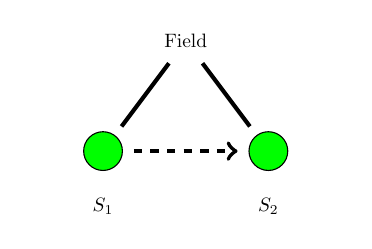
\begin{tikzpicture}[scale=.7,transform shape,
        pfeil/.style={shorten <=4pt, shorten >=4pt, line width=1.5pt},
        mytext/.style={text width=2.5cm,align=center}]
    \node[draw,fill=green,minimum size=2em] at (0,0) [circle] (A0) {};
    \node[draw,fill=green,minimum size=2em] at (3,0) [circle] (A1) {};
    \node at (1.5,2) [rectangle] (A2) {Field};
    \node[mytext,below of = A0] {$S_1$};
    \node[mytext,below of = A1] {$S_2$};
    \draw[pfeil,->,dashed] (A0)--(A1) ;
    \draw[pfeil,-] (A0)--(A2) ;
    \draw[pfeil,-] (A2)--(A1) ;
    \end{tikzpicture}
\end{center}

\end{frame}

\begin{frame}{Resources, Tools and State Changes} 

At the same time, in the systemic abstraction, the materiality of the
\emph{tool} is pushed back further in favour of the concept of \emph{action}
and a component concept is prepared as proposed by C. Szyperski for Component
Software.

There, \emph{components} are basically conceptualised as \emph{stateless} with
all the resulting consequences. In contrast to this \emph{objects} are
conceptualised as state-bearing units of instantiation to maintain a certain
standardisation of workpieces required for a repeated application of a
function within a production process.

\end{frame}

\begin{frame}{Resources, Tools and State Changes}

A similar idea comes through when Souchkov describes the two goals of
\emph{Resource Analysis} as essential component of TRIZ:
\begin{itemize}
\item Analysis of the resources that are to be \emph{treated or consumed} in
  the course of a process,
\item and analysis of the resources that can be \emph{used} to carry out the
  process or to solve the problem,
\end{itemize}
i.e., he distinguishes resources of the first kind, which undergo
state-changing transformations as \emph{workpieces} and resources of the
second kind, which are used as tools to \emph{mediate} these state changes.

\end{frame}

\begin{frame}{Operation and Maintenance of Technical Systems} 

Such a notion also corresponds well with the widespread organisation of
production processes, where a distinction is made between operating and
maintenance mode.

In the operating mode, the focus is on the functional properties of the tool,
while in the maintenance mode its material properties are focused.

As an independent technical system in a narrower sense, only the
operating mode is modelled as the target of a "problem solution".

The maintenance mode is part of the supersystem, which is concerned with the
\emph{reproduction} of the tools as \emph{resources} used in the operating
mode.

\end{frame}

\begin{frame}{Operation and Maintenance of Technical Systems} 

In the (classical) operating mode the focus is on the use of tools and
the material throughput of workpieces, which are thereby transformed into
useful products, in many cases \emph{technical artefacts}, which are either
further processed as semi-finished products in a following technical system or
enter into such contexts as tools themselves.

In both cases the useful product is a \emph{resource} for further systemic
processes.

But TRIZ is not (primarily) about system analysis but about \emph{problem
  solving} and the design of viable technical systems in a \emph{systemic
  development} \textbf{process}.

\end{frame}

\begin{frame}{Systemic Development and Problem Solving}
  
Souchkov clarifies the role of \emph{Resource Analysis} in such a process:
\begin{quote}\small
  A technical system has different resources at its disposal for the
  completion of its function. A function can only be completed using suitable
  resources. Resources are therefore elementary building blocks of a problem
  solution. The skilful use of resources distinguishes an efficient from an
  inefficient system.
\end{quote}

The question of systemic operating conditions is thus reversed -- it is not
about what conditions are \emph{required} for the operation of a particular
system, but what kind of system under \emph{given} operating conditions
promises an efficient problem solution.

The focus thus shifts from the operating conditions of an existing system to
the question of a systemic development and co-evolution in a given context.

\end{frame}

\end{document}
